\documentclass{article}

\usepackage{arxiv}

\usepackage[utf8]{inputenc} % allow utf-8 input
\usepackage[T1]{fontenc}    % use 8-bit T1 fonts
\usepackage{hyperref}       % hyperlinks
\usepackage{url}            % simple URL typesetting
\usepackage{booktabs}       % professional-quality tables
\usepackage{amsfonts}       % blackboard math symbols
\usepackage{amsmath}
\usepackage{nicefrac}       % compact symbols for 1/2, etc.
\usepackage{microtype}      % microtypography
\usepackage{graphicx}
\usepackage{array}
\usepackage{longtable}
\usepackage[numbers,square,sort&compress]{natbib}

\title{Bitres: A Decentralized Stablecoin System Collateralized by Bitcoin}
\author{Invariant Core\\
\texttt{invariantcore@gmail.com}\\
\url{https://www.bitres.org}}
\date{\today}

\renewcommand{\shorttitle}{Bitres: A Decentralized Stablecoin System Collateralized by Bitcoin}
\renewcommand{\headeright}{}
\renewcommand{\undertitle}{}

\hypersetup{
  colorlinks=true,
  linkcolor=blue,
  citecolor=blue,
  urlcolor=blue,
  pdftitle={Bitres: A Decentralized Stablecoin System Collateralized by Bitcoin},
  pdfauthor={Invariant Core}
}

\setlength{\parindent}{2em}
\setlength{\parskip}{0pt}

\begin{document}

\maketitle

\begin{abstract}
The global monetary system has gradually transitioned from commodity-backed money to fiat currencies supported by sovereign credit. While fiat systems provide short-term price stability and transactional convenience, their long-term purchasing power remains vulnerable to persistent monetary expansion. Bitcoin emerged as a decentralized alternative, restoring scarcity, trustless settlement, and monetary immutability. Over time, Bitcoin has increasingly functioned as digital gold---a global store of value and settlement asset---yet its price volatility limits its current role as a medium of everyday exchange.

In this paper, we propose the Bitcoin Reserve System (Bitres), a Bitcoin-native monetary framework designed to bridge the gap between Bitcoin's long-term monetary properties and the short-term stability required for economic activity. Bitres introduces a stablecoin system fully collateralized by Bitcoin and anchored to a conceptual unit of account, referred to as Ideal USD. The system employs a three-token structure, consisting of a stablecoin (BTD), a bond token (BTB), and a governance token (BRS), to distribute risk across multiple layers while preserving Bitcoin as the ultimate source of value.

By combining Bitcoin's monetary discipline with market-based stabilization mechanisms, Bitres seeks to enhance Bitcoin's practical usability without compromising its core principles. Viewed as a transitional monetary layer rather than a replacement, Bitres provides a pathway toward a future monetary system in which Bitcoin can more fully realize its original vision as sound, peer-to-peer electronic money, including the potential evolution toward Bitcoin-native units of account under suitable conditions.
\end{abstract}

\keywords{Stablecoin \and Bitcoin \and DeFi \and Cryptocurrency}

\section{Introduction}

In today's world, the US dollar is undoubtedly the world currency, marketed globally based on the credit of the United States alone. The hegemony of the US dollar began with the Bretton Woods system established in 1944\citep{bordo1993bretton}, which is less than a hundred years ago. In this system, the US dollar was pegged to gold, and other countries' currencies were pegged to the US dollar, with 1 US dollar containing 0.88867 grams of gold. However, the Bretton Woods system began to collapse in 1971, and since then the US dollar is no longer a gold-backed currency, thus entering an era of massive money printing and beginning decades of rapid expansion. The gold content of the US dollar has depreciated repeatedly, from 0.88867 grams of gold to 0.00647 grams (in October 2025, gold reached a historical high of \$4,381 per ounce), a shrinkage of 99.27\%. If we view the US dollar as an altcoin, it has experienced a severe long-term depreciation relative to gold.

In the post-Bretton Woods era, the collateral for the US dollar is US Treasury bonds, and the scale of US debt has grown from \$0.4 trillion in 1971 to \$38 trillion in 2025\citep{ustreasury2024debt}, an expansion of nearly a hundred times. US Treasury bonds have become the eternal power source of the US dollar printing press. Can this perpetual motion machine model of unlimited debt issuance continue forever? Ultimately, the debt repayment capacity of US Treasury bonds comes from future printed US dollars, and the actual purchasing power of these dollars is determined by America's production capacity, by America's GDP, by America's military strength, and by America's influence in the hearts of people around the world.

Since the 2008 financial crisis, America's comprehensive national strength has begun to decline, and the COVID-19 pandemic in 2020 further accelerated this process. The scale of US Treasury bonds that it can support in the future must also have an upper limit. There exists a non-negligible risk that the expanding US Treasury bond market may eventually face a systemic adjustment, as the ever-increasing scale of US debt issuance collides with the gradually declining overall credit of the United States. Under such a scenario, the US dollar could experience significant inflationary pressure and depreciation.

It was precisely because of the US dollar's problems of centralized control, excessive inflation, and susceptibility to political influence that Satoshi Nakamoto proposed the Bitcoin system in 2008: a cryptocurrency system with a fixed total supply that will never be inflated\citep{nakamoto2008bitcoin}. Although Bitcoin has only been born for 17 years, it has already achieved significant success, being recognized as ``digital gold'' with a market capitalization exceeding \$2 trillion. Fundamentally, the Bretton Woods system collapsed only 54 years ago, and the US dollar's history as a purely uncollateralized fiat currency is only half a century. In contrast, gold has served as the world's currency for thousands of years. Nations are perishable, but gold is immortal, and Bitcoin may be considered even more durable than gold, given its fixed supply and cryptographic immutability. Therefore, as an upgraded digital version of gold, Bitcoin can completely serve as the cornerstone of a new generation of monetary systems, playing in the next millennium the role that gold played in the previous millennium. A monetary system built on Bitcoin will be more enduring than one built on national credit.

Satoshi Nakamoto's original intention in creating Bitcoin was to build a peer-to-peer electronic cash system, and it has already achieved tremendous success. However, because its total supply is fixed and cannot be adjusted according to market demand, people tend to hoard rather than use it. Therefore, Bitcoin has only partially fulfilled its original role at the current stage, becoming a peer-to-peer electronic gold system. This paper believes that in the future, as Bitcoin's price volatility against fiat currencies gradually decreases and its exchange ratio against a basket of goods becomes increasingly stable, Bitcoin will eventually realize Satoshi Nakamoto's vision and become a widely used electronic currency. Imagine when Bitcoin's price rises to \$1 million, 1 satoshi will be exactly 1 cent, and 100 satoshis will be \$1. At that time, people will be able to conveniently use Bitcoin for daily payments and transactions.

Of course, to achieve this goal, a necessary condition must be met: a high-speed Bitcoin Layer 2 chain, because the Bitcoin mainnet's throughput is too low and block confirmation time is too long to meet large-scale payment needs. In the future, when a certain Bitcoin Layer 2 chain matures, with the mainnet serving as the settlement layer and the Layer 2 chain serving as the payment layer, Bitcoin can completely become a globally universal electronic cash. Of course, economists will still argue that Bitcoin is a deflationary currency and is not suitable as a daily circulating currency because people will tend to hoard rather than spend. In response, we believe that an inflationary currency pegged to Bitcoin can be designed on the Layer 2 chain, initially with 1 inflationary currency = 100 satoshis, and then increasing its supply by 2\% annually, thereby achieving moderate inflation to meet economic development needs.

Of course, the above vision requires the continued expansion of Bitcoin consensus and the maturation of Bitcoin Layer 2 chains to gradually realize. Before reaching the shore that Satoshi Nakamoto described for us, the world still needs a stablecoin collateralized by Bitcoin as a transition, which can adopt monetary policies similar to the Federal Reserve, allowing it to flexibly adjust supply according to market demand while maintaining moderate inflation to meet economic development needs. Currently, stablecoins issued based on BTC in the crypto space include only a few such as USDS, with a scale of less than \$10 billion, accounting for less than 0.5\% of Bitcoin's \$2 trillion market capitalization. There is still significant credit space to create new currencies.

Based on this, we combine the advantages of Bitcoin and fiat currencies to create a new type of monetary system: the Bitcoin Reserve System, hereafter referred to as Bitres. This system hopes to complete the other half of Satoshi Nakamoto's puzzle during the transition phase by issuing stablecoins collateralized by Bitcoin and introducing monetary policies to adjust its supply, exchange rates, interest rates, and other parameters. This enables the stablecoin to obtain a solid value foundation from Bitcoin while also having the advantage of US dollar price stability, serving as a bridge to realize Satoshi Nakamoto's vision: a peer-to-peer electronic cash system.

\section{Ideal USD}

In 2200, humanity has colonized Mars, and the currency used in interstellar transactions has long since become Bitcoin. This science fiction-like imagination may come true within a century, but when we shift our gaze from future Mars back to today's Earth, we must admit that US dollar credit is still deeply ingrained at this stage. Bitcoin has only been born for a little over a decade, and compared to the mission it will bear for the next millennium, it is still in its infancy, with relatively high price volatility and a scale that is still relatively small compared to US Treasury bonds. In 2025, developing a system completely unrelated to the US dollar, with exchange rates directly pegged to BTC, will not be recognized by the market and will be considered an unstable risky asset rather than a stablecoin, making it impossible to realize Satoshi Nakamoto's true vision of electronic cash.

Therefore, when the timing is not yet mature, we need to make certain compromises: in the initial phase of the Bitres, the stablecoin will still be pegged to the US dollar, but not the real US dollar---rather the Ideal USD. In the more distant future, when Bitcoin's total market capitalization grows large enough, perhaps comparable to the scale of US Treasury bonds, the Bitres may decouple from the US dollar and transition to a pure Bitcoin system.

\subsection{Fisher Equation}

Regarding what Ideal USD is, we will begin our analysis from a basic equation about the quantity of money. We all know that the Fisher equation describes the relationship between the quantity of money and the price level\citep{fisher1911purchasing}:

\begin{equation}
MV = PT
\end{equation}

Where $M$ represents the quantity of money, $V$ represents the velocity of money circulation, $P$ represents the weighted average price level, and $T$ represents the total volume of transactions of various goods. From this equation, we can easily derive that when $V$ and $T$ remain constant, $M$ and $P$ are directly proportional. That is to say, the more money is created, the more prices will rise accordingly, which is so-called inflation.

Friedman once proposed a fixed ``monetary rule,'' namely Friedman's k-percent rule, advocating that the money supply should automatically grow at a fixed rate each year\citep{friedman1960program}. However, this rule has two difficulties. First, the velocity of money circulation $V$ is not fixed and is difficult to measure in practice. Thus, even if $M$ grows at a fixed rate each year, changes in $V$ may cause abnormal price fluctuations. Second, economic development does not grow at a fixed rate each year either---GDP growth rates may be sometimes high and sometimes low, causing unpredictable changes in $T$. When the economy develops rapidly, the amount of money increased at a fixed growth rate k is insufficient to meet market demand, causing deflation; when the economy grows slowly or even contracts, the fixed growth in money supply will cause even higher inflation.

It is precisely because $V$ and $T$ are difficult to measure that directly adjusting the money supply has an unclear impact on prices. Therefore, in practice, it is better for monetary policy to directly target the inflation rate, that is, to focus only on the price level indicator $P$ in the Fisher equation.

\subsection{Calculation of Ideal USD}

In today's world, major central banks basically adopt inflation targeting as their main monetary policy, with annual inflation targets generally set at 2\%\citep{fomc2012statement}. However, due to political interference, economic disruptions, unemployment considerations, and bailout considerations, central banks cannot consistently implement this target. Therefore, in some years, extremely high inflation rates occur, deviating from the 2\% target.

\begin{figure}[h]
\centering
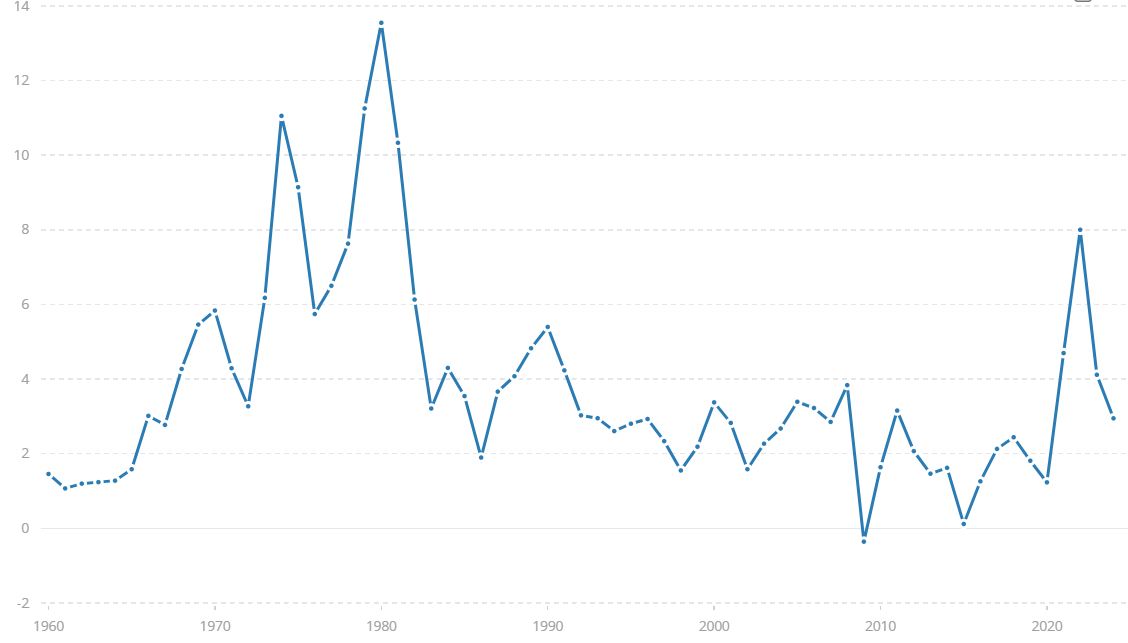
\includegraphics[width=0.8\textwidth]{images/image1.png}
\caption{US Inflation Rate (1960--2024)\citep{worldbank2024inflation}}
\label{fig:inflation}
\end{figure}

The World Bank provides US annual inflation rate data from 1960 to 2024\citep{worldbank2024inflation}, as shown in Figure~\ref{fig:inflation}. From Figure~\ref{fig:inflation}, we can see that since 1960, the US inflation rate has often deviated from 2\%, especially during the 1970s--1980s when inflation reached as high as 13.5\%, followed by the post-2020 pandemic period when inflation reached 8\%.

Compared to the real US dollar, whose inflation rate often deviates from the 2\% target, we define Ideal USD as follows:

\textbf{Ideal USD}: A dollar with a fixed annual inflation rate of 2\%.

Ideal USD serves as a conceptual unit of account rather than a claim on real-world fiat currency.

We will next calculate the exchange rate relationship between Ideal USD and real USD. Let the month when the Bitres officially launches be the initial month. Let the Personal Consumption Expenditures Price Index in the initial month be $\text{PCE}_0$, and the Personal Consumption Expenditures Price Index in the current month be $\text{PCE}_n$, where $n$ represents the $n$-th month after the initial month.

We can obtain the IUSD to USD exchange rate as:

\begin{equation}
\text{IUSD/USD} = \frac{\text{PCE}_n}{\text{PCE}_0\times1.02^{n/12}}
\label{eq:iusd-usd}
\end{equation}

Note: All exchange rates in this paper are expressed in the form A/B, representing the ratio of exchanging token A for token B.

Based on inflation data published by the US government, we plot the exchange rate of Ideal USD against real USD, as shown in Figure~\ref{fig:iusd-usd}. From Figure~\ref{fig:iusd-usd}, we can see that over more than 60 years, Ideal USD has appreciated about 3 times relative to real USD, meaning real USD has depreciated about 66\% against Ideal USD.

\begin{figure}[h]
\centering
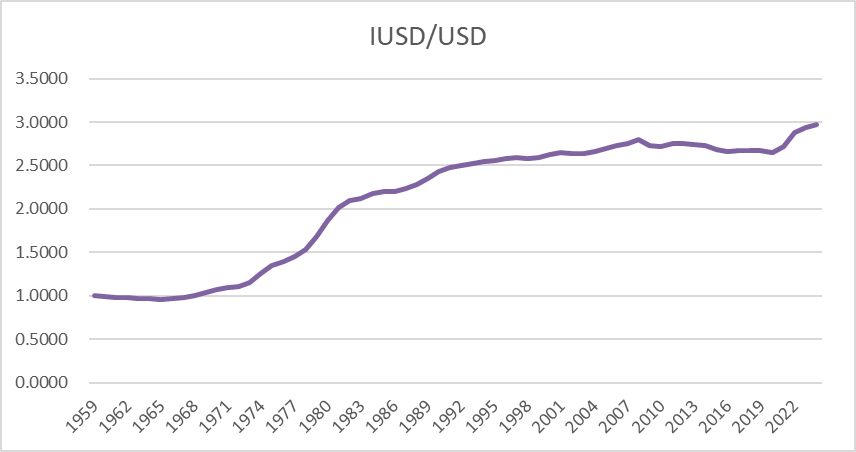
\includegraphics[width=0.8\textwidth]{images/image2.png}
\caption{Exchange Rate of Ideal USD to Real USD (1959--2024)}
\label{fig:iusd-usd}
\end{figure}

\section{Core Mechanisms of the Bitres}

The Bitres is a three-token system, consisting of a stablecoin, a bond token, and a governance token. Their names and abbreviations are as follows:

\begin{itemize}
\item Stablecoin: Bitcoin Dollar, abbreviated as BTD;
\item Bond Token: Bitcoin Bond, abbreviated as BTB;
\item Governance Token: Bitres Token, abbreviated as BRS.
\end{itemize}

The modern Federal Reserve System mainly issues US dollars collateralized by US Treasury bonds, with its balance sheet shown in Table~\ref{tab:fed-balance}. The Bitres issues Bitcoin Dollars collateralized by Bitcoin, with its balance sheet shown in Table~\ref{tab:brs-balance}. The credit of the US dollar comes from the credit of US Treasury bonds, which is essentially the credit of the US government, while the credit of Bitcoin Dollar comes from the credit of BTC, which is essentially the credit of mathematics.

\begin{table}[h]
\centering
\caption{Simplified Federal Reserve Balance Sheet}
\label{tab:fed-balance}
\begin{tabular}{c|c}
\toprule
Assets & Liabilities \\
\midrule
US Treasury Bonds & USD \\
\bottomrule
\end{tabular}
\end{table}

\begin{table}[h]
\centering
\caption{Bitres Balance Sheet}
\label{tab:brs-balance}
\begin{tabular}{c|c}
\toprule
Assets & Liabilities \\
\midrule
BTC & BTD \\
& BTB \\
\bottomrule
\end{tabular}
\end{table}

\subsection{Anchor and Collateral Ratio}

In Section 2, we have designed the Ideal USD that changes according to a 2\% inflation rate. Ideal USD is the anchor for the stablecoin of the Bitres, meaning BTD will strive to be pegged to Ideal USD:

\begin{equation}
1 \;\text{BTD} =1 \;\text{IUSD}
\label{eq:btd-iusd}
\end{equation}

The calculation formula for IUSD is shown in Equation~(\ref{eq:iusd-usd}).

After new inflation data is released, the exchange rate of Ideal USD to real USD will be recalculated and updated. Once we have the price of Ideal USD, we can calculate the collateral ratio of the Bitres. The collateral ratio is defined as the ratio of the total value of BTC in the treasury to the total value of all BTD. The collateral ratio essentially represents the BTC value backing each BTD, and its calculation formula is shown in Equation~(\ref{eq:collateral-ratio}):

\begin{equation}
\text{Collateral Ratio} = \frac{\text{Total BTC Value}}{\text{Total BTD Value}} = \frac{\text{Total BTC Amount} \times \text{BTC Price}}{\text{Total BTD Amount} \times \text{IUSD Price}}
\label{eq:collateral-ratio}
\end{equation}

Where BTC price and IUSD price are denominated in USD. All prices mentioned hereafter refer to USD-denominated prices.

\subsection{Pegging Mechanism}

The goal of the Bitres is to achieve 1 BTD = 1 IUSD. The pegging mechanism is shown in Figure~\ref{fig:anchor}.

\begin{figure}[h]
\centering
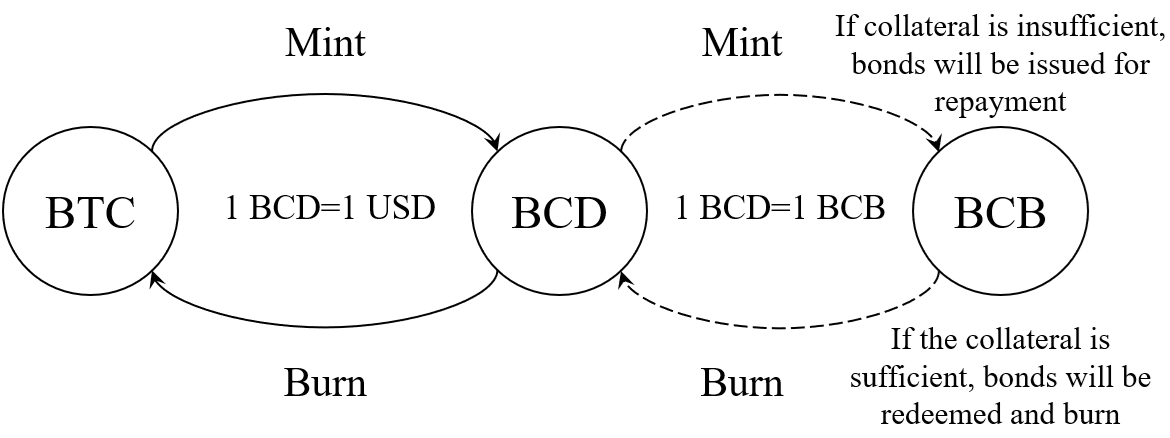
\includegraphics[width=0.8\textwidth]{images/image3.png}
\caption{Pegging Mechanism}
\label{fig:anchor}
\end{figure}

\textbf{Core Pegging Mechanism}: The system always values 1 BTD as 1 IUSD. When BTC is deposited into the treasury, BTD is minted at the real-time exchange rate; conversely, when BTD is sent to the system, the BTD will be burned, and BTC is redeemed at the real-time exchange rate. If the collateral ratio is insufficient, the system will mint bond token BTB to make up the difference. When the collateral ratio becomes sufficient again, BTB can be exchanged 1:1 for BTD. The system specifies a minimum price $\text{P}_\text{minBTB}$ for BTB. When BTB's market price falls below this minimum price, the system will only mint BTB at the minimum price. This creates a secondary shortfall when repaying BTD, which will be finally compensated using the BRS reserved in the system.

During deep bear markets, when BTC price drops significantly, causing the collateral ratio to fall well below 100\%, redemption of BTD at this time will yield a certain amount of BTC plus large amounts of BTB and BRS. If the bear market lasts too long and depletes all the BRS in the system, temporary depegging will occur, causing 1 BTD $<$ 1 IUSD. However, this depegging will not be like the death spiral that Terra experienced\citep{terra2022collapse}, where both UST and Luna fell endlessly. Unlike uncollateralized algorithmic stablecoins such as Terra, which rely solely on reflexive mint-and-burn dynamics, BTD is a stablecoin collateralized by Bitcoin. Each BTD is backed by BTC. As long as BTC does not go to zero, BTD will not go to zero either. When market panic subsides or Bitcoin emerges from the bear market, BTD will re-peg to IUSD.

In addition to ensuring price stability, the Bitres's minting and burning mechanism can also adjust BTD supply according to market demand: when users have demand for BTD, they can use BTC to mint new BTD; when the market doesn't need as much BTD, users can burn BTD to redeem BTC. The minting and burning mechanisms are described in detail below.

\subsection{Minting}

When users deposit BTC into the treasury, the system will mint a corresponding amount of BTD according to the exchange rate. The BTC to BTD exchange rate is shown in Equation~(\ref{eq:btc-btd-rate}):

\begin{equation}
\text{BTC/BTD} =\frac{\text{BTC Price}}{\text{IUSD Price}}
\label{eq:btc-btd-rate}
\end{equation}

The minting process is shown in Figure~\ref{fig:mint}.

\begin{figure}[h]
\centering
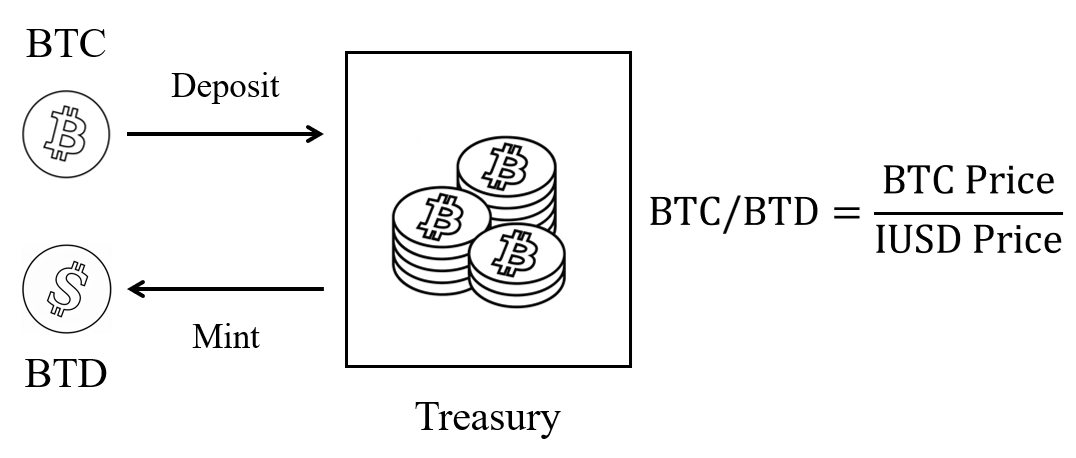
\includegraphics[width=0.6\textwidth]{images/image4.png}
\caption{Minting Process}
\label{fig:mint}
\end{figure}

\subsection{Redemption}

When users deposit BTD back into the treasury, the system will burn the corresponding BTD and return the appropriate amount of BTC to the user according to the exchange rate. This is divided into three cases depending on whether the collateral ratio is greater than 100\% and whether BTB's market price is below the system-specified minimum.

\subsubsection{Collateral Ratio $\geq$ 100\%}

At this time, the BTC in the treasury is sufficient, and its total value is enough to repay all BTD. During redemption, each BTD can receive a sufficient amount of BTC at the Ideal USD price. The redemption process is shown in Figure~\ref{fig:redeem-normal}.

\begin{figure}[h]
\centering
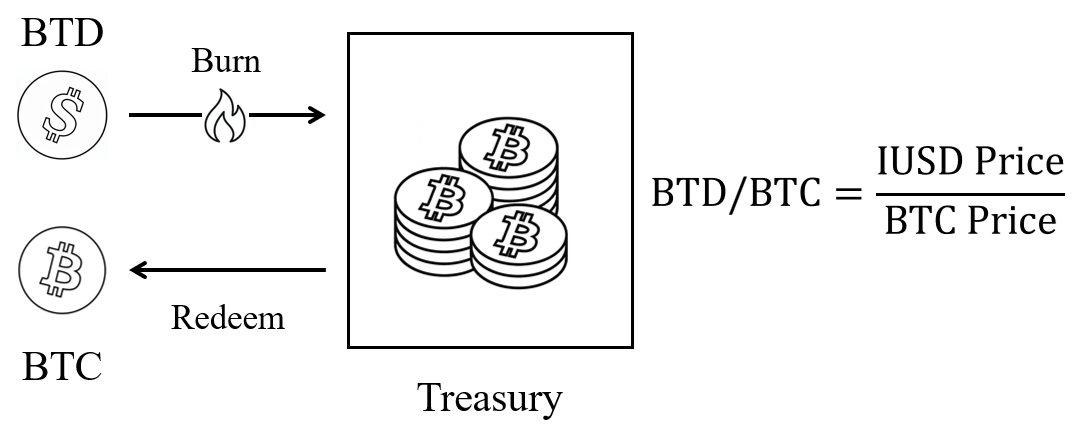
\includegraphics[width=0.6\textwidth]{images/image5.png}
\caption{Redemption Process (Collateral Ratio $\geq$ 100\%)}
\label{fig:redeem-normal}
\end{figure}

\subsubsection{Collateral Ratio $<$ 100\% and BTB Price $\geq$ Minimum Price}

When BTC price drops such that total BTC value $<$ total BTD value, the collateral ratio is below 100\%. The amount of BTC each BTD can receive is Total BTC Amount / Total BTD Amount, which is insufficient to repay 1 BTD. The difference between the two is called the primary shortfall, as shown in Equation~(\ref{eq:first-gap}):

\begin{equation}
\text{Primary Shortfall}={ (1-\text{Collateral Ratio})\times\text{IUSD Price}}
\label{eq:first-gap}
\end{equation}

This shortfall will be compensated by minting bond token BTB.

Thus, when the collateral ratio is insufficient, each BTD redeemed yields both $x$ BTC and newly minted $y$ BTB, as shown in Equation~(\ref{eq:redeem-btb}):

\begin{equation}
1 \text{ BTD} = x \text{ BTC} + y \text{ BTB}
\label{eq:redeem-btb}
\end{equation}

Where $x = \frac{\text{Total BTC Amount}}{\text{Total BTD Amount}}$, $y =\frac{ (1-\text{Collateral Ratio})\times\text{IUSD Price}}{\text{BTB Price}}$. The redemption process is shown in Figure~\ref{fig:redeem-btb}.

\begin{figure}[h]
\centering
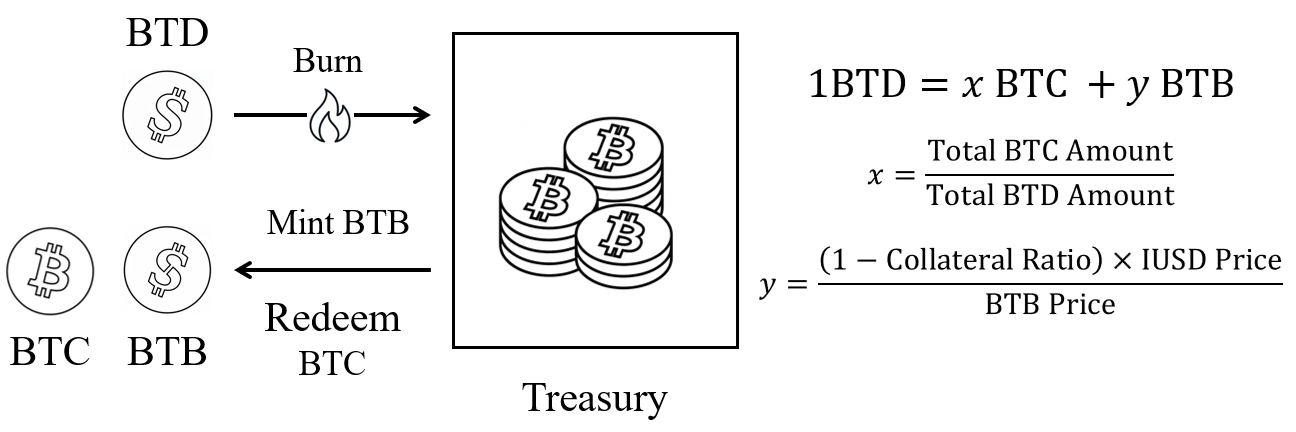
\includegraphics[width=0.75\textwidth]{images/image6.png}
\caption{Redemption Process (Collateral Ratio $<$ 100\% and BTB Price $\geq$ Minimum Price)}
\label{fig:redeem-btb}
\end{figure}

BTB is a bond token representing the future right to redeem stablecoin BTD. When the collateral ratio exceeds 100\% again in the future, bond redemption will be opened, and BTB can be redeemed 1:1 for BTD, as shown in Equation~(\ref{eq:btb-btd}):

\begin{equation}
1 \;\text{BTB} =1 \;\text{BTD}
\label{eq:btb-btd}
\end{equation}

BTB redemption follows a first-come-first-served principle. The redeemable quota is $(\text{Collateral Ratio}-1) \times \text{Total BTD}$. When the quota is exhausted, the collateral ratio drops back to 100\%, and redemption is no longer possible until the collateral ratio exceeds 100\% again in the future. Table~\ref{tab:btb-operations} illustrates the BTB operation mechanism under different collateral ratios.

\begin{table}[h]
\centering
\caption{BTB Operation Mechanism Under Different Collateral Ratios}
\label{tab:btb-operations}
\begin{tabular}{c|c|c|c}
\toprule
Collateral Ratio & BTB Operation & Redeemable & Redemption Quota \\
\midrule
$\geq$100\% & Collect and Burn & Yes & $(\text{Collateral Ratio}-1) \times \text{Total BTD}$ \\
$<$100\% & Mint and Issue & No & 0 \\
\bottomrule
\end{tabular}
\end{table}

\subsubsection{Collateral Ratio $<$ 100\% and BTB Price $<$ Minimum Price}

Since BTB price is entirely determined by the market, market panic, insufficient liquidity, or price manipulation by arbitrageurs may cause extremely low BTB prices. If BTB is minted at this market price to compensate for the BTD shortfall, a large or even massive amount of BTB will be minted, creating enormous future bond repayment pressure on the system and potentially causing system failure in severe cases. This can be seen from the Luna collapse event. Due to market panic during the bear market, after UST depegged, an astronomical amount of Luna tokens were minted in an attempt to maintain UST's price stability. Ultimately, this effort failed, and both Luna and UST prices spiraled downward in a death spiral. If the project team had not ultimately shut down the minting function, it is unknown how far prices could have fallen.

To avoid this unlimited minting, the system has designed a price protection mechanism for BTB, setting a minimum price $\text{P}_\text{minBTB}$ for BTB. When BTB's market price falls below $\text{P}_\text{minBTB}$, the system will only use $\text{P}_\text{minBTB}$ as the minting price for BTB, rather than the market price. At this point, when a user redeems 1 BTD, after receiving BTC from the treasury and newly minted BTB from the system, there will still be a secondary shortfall that has not been fully compensated, as shown in Equation~(\ref{eq:second-gap}):

\begin{equation}
\text{Secondary Shortfall}=\frac{ (1-\text{Collateral Ratio})\times\text{IUSD Price}\times(\text{P}_\text{minBTB}-\text{BTB Price})}{\text{P}_\text{minBTB}}
\label{eq:second-gap}
\end{equation}

The secondary shortfall will be compensated using the BRS reserved in the system.

Thus, when the system's collateral ratio is insufficient and BTB price is below the minimum price, each BTD redeemed yields $x$ BTC, newly minted $y$ BTB, and $z$ BRS, as shown in Equation~(\ref{eq:redeem-brs}):

\begin{equation}
1 \text{ BTD} = x \text{ BTC} + y \text{ BTB}+ z \text{ BRS}
\label{eq:redeem-brs}
\end{equation}

Where $x = \frac{\text{Total BTC Amount}}{\text{Total BTD Amount}}$, $y =\frac{ (1-\text{Collateral Ratio})\times\text{IUSD Price}}{\text{P}_\text{minBTB}}$, $z =\frac{ y\times(\text{P}_\text{minBTB}-\text{BTB Price})}{\text{BRS Price}}$. The redemption process is shown in Figure~\ref{fig:redeem-brs}.

\begin{figure}[h]
\centering
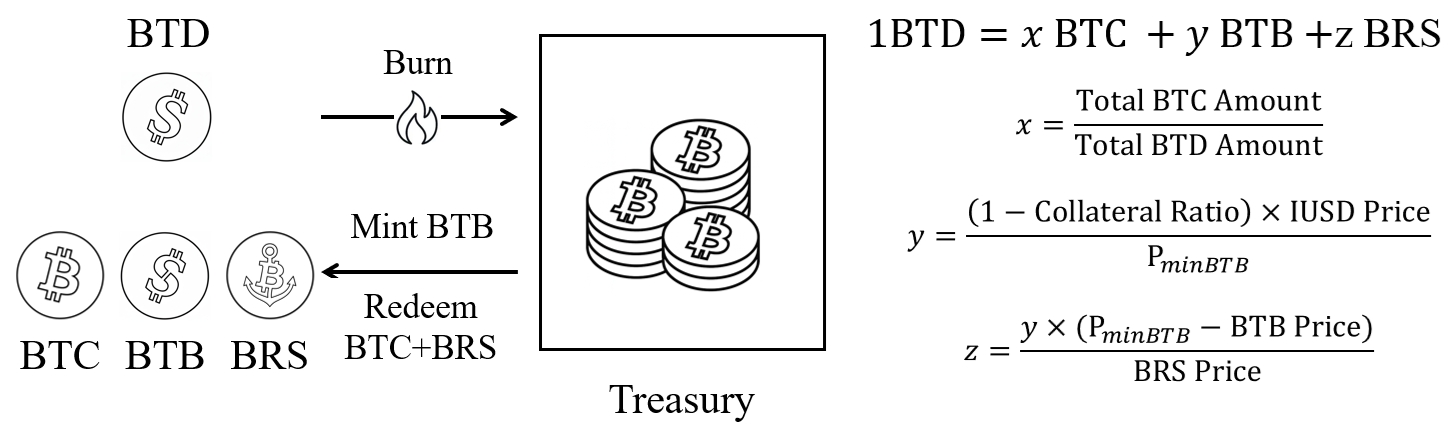
\includegraphics[width=0.9\textwidth]{images/image7.png}
\caption{Redemption Process (Collateral Ratio $<$ 100\% and BTB Price $<$ Minimum Price)}
\label{fig:redeem-brs}
\end{figure}

\subsection{Mining}

BRS is the governance token of the Bitres. It will have a fixed total supply and be distributed through mining similar to Bitcoin's four-year halving mechanism. Half of the BRS tokens will be distributed in the first four years, half of the remainder in the next four years, and so on. Specific distribution forms include liquidity mining, single-token staking mining, and preset address distribution.

BRS tokens have the following rights:

\textbf{Governance Rights}: Holders can vote to determine adjustments to governable parameters and governable smart contracts in the Bitres;

\textbf{Fee Buyback}: When users perform various system operations, a certain fee is charged (detailed in Section 5), which is used to buy back BRS;

In addition to the above two rights, BRS tokens also have residual equity in the system, as shown in Equation~(\ref{eq:equity}):

\begin{equation}
\text{Owner's Equity} = \text{Net Assets} = \text{Total BTC Value} - \text{Total BTB Value} - \text{Total BTD Value}
\label{eq:equity}
\end{equation}

The net assets corresponding to each BRS is called net asset value per token, as shown in Equation~(\ref{eq:brs-nav}):

\begin{equation}
1 \text{ BRS} = \frac{\text{Total BTC Value} - \text{Total BTB Value} - \text{Total BTD Value}}{\text{Total BRS Amount}}
\label{eq:brs-nav}
\end{equation}

It is easy to see that when the total collateral ratio (including BTB liabilities) is less than 100\%, net assets are negative. However, this does not mean BRS tokens have no value, because the value of BRS tokens also comes from the brand value of the entire system and future fee income.

\section{Interest Rates}

There are two important interest rates in the Bitres: deposit rate and bond rate. The deposit rate refers to the interest rate for users staking their BTD in the system. The bond rate refers to the interest rate for users staking their BTB in the system. After users deposit tokens into the system, they can earn staking interest over time according to the applicable rate. All interest rates described in this section are algorithmic policy variables rather than contractual guarantees.

\subsection{Deposit Rate}

The deposit rate is determined by the market, with the basic goal of making the stablecoin price as close as possible to the Ideal USD price. The specific strategy is: when BTD's market price is less than IUSD's price and continues to fall, the system raises the deposit rate to increase attractiveness; when BTD's market price is greater than IUSD's price and continues to rise, the system lowers the deposit rate. The ultimate target range for stablecoin price control is 0.99--1.01 IUSD. When the stablecoin price is within this range, the deposit rate remains unchanged.

The specific deposit rate adjustment mechanism is shown in Table~\ref{tab:deposit-rate}.

\begin{table}[h]
\centering
\caption{Deposit Rate Policy}
\label{tab:deposit-rate}
\begin{tabular}{c|c|c}
\toprule
BTD Price Range & Price Movement & Rate Policy \\
\midrule
$<$0.99 IUSD & Falling & Raise Rate \\
$<$0.99 IUSD & Rising & Unchanged \\
{[0.99 IUSD, 1.01 IUSD]} & Either & Unchanged \\
$>$1.01 IUSD & Falling & Unchanged \\
$>$1.01 IUSD & Rising & Lower Rate \\
\bottomrule
\end{tabular}
\end{table}

\subsection{Bond Rate}

The bond rate is determined by the market, with the basic goal of making the bond price as close as possible to the stablecoin price. The specific strategy is: when BTB's market price is less than BTD's market price and continues to fall, the system raises the bond rate to increase attractiveness; when BTB's market price is greater than BTD's market price and continues to rise, the system lowers the bond rate. The ultimate target range for bond price control is 0.99--1.01 BTD. When the bond price is within this range, the bond rate remains unchanged.

The specific bond rate adjustment mechanism is shown in Table~\ref{tab:bond-rate}.

\begin{table}[h]
\centering
\caption{Bond Rate Policy}
\label{tab:bond-rate}
\begin{tabular}{c|c|c}
\toprule
BTB Price Range & Price Movement & Rate Policy \\
\midrule
$<$0.99 BTD & Falling & Raise Rate \\
$<$0.99 BTD & Rising & Unchanged \\
{[0.99 BTD, 1.01 BTD]} & Either & Unchanged \\
$>$1.01 BTD & Falling & Unchanged \\
$>$1.01 BTD & Rising & Lower Rate \\
\bottomrule
\end{tabular}
\end{table}

Both the deposit rate and bond rate have a system maximum rate cap to prevent rates from spiking to uncontrollable heights under extreme market conditions, which would mint astronomical amounts of BTD or BTB and bring unacceptable risks to the system.

\section{Fees}

The Bitres supports long-term system operation and BRS value growth through fee collection. Fees also prevent hacker attacks and malicious arbitrage. The system has the following main types of fees:

\subsection{Minting Fee}

When users use BTC to mint BTD, the system charges a certain percentage as a minting fee. This fee is deducted from the newly minted BTD, and users receive BTD after the fee deduction. The minting fee rate is initially set at a low percentage and can later be adjusted through governance.

\subsection{Redemption Fee}

When users redeem BTD for BTC, the system charges a certain percentage as a redemption fee. This fee is deducted from the BTC the user should receive, and the BTC after deduction is returned to the user. The redemption fee rate is initially set at a low percentage and can also be adjusted through governance later.

\subsection{Interest Fee}

In addition to direct operational fees, the system also collects interest fees from the interest pool. The specific mechanism is as follows:

Each day, the system calculates the total interest generated by all staked BTD from the previous day. Then, the system collects a certain percentage as interest fee from this interest. This fee is not directly deducted from each user's interest, but is realized by minting new BTD, which enters the treasury.

\subsection{Fee Usage}

All collected fees go into the treasury and are mainly used for the following purposes:

\textbf{BRS Buyback}: The treasury will periodically use collected fees to buy back BRS on the market. The bought-back BRS is stored in the treasury, which helps increase BRS's value and scarcity.

\textbf{System Reserve}: The BRS in the treasury also serves as system reserve funds, used to meet compensation demands under extreme market conditions and enhance the system's risk resistance.

\textbf{Ecosystem Development}: With governance approval, a portion of fees can be used to support the development of the Bitres ecosystem, such as developer incentives, security audits, etc.

\section{Risks}

To maintain the price peg between stablecoin BTD and Ideal USD, the Bitres has set up triple asset protection. The first layer is the BTC reserved in the treasury, the second layer is the BTB minted by the system, and the third layer is the BRS reserved in the treasury. Of course, BTD's price support essentially comes from BTC's value, but since BTC price is always fluctuating, when BTC price drops causing the collateral ratio to fall below 100\%, bond token BTB is needed to compensate for the price gap at that time to resist risk. If BTB's market price also drops too much, falling below the set minimum price, BRS is still needed to compensate for the remaining price gap.

For participants, holding BTD is relatively lower-risk because there are multiple guarantees ensuring price pegging, but its investment returns are also relatively low, and it is mainly used as a stablecoin. Holding BTB is moderately safe. The risk borne by holders is that when the collateral ratio is below 100\%, BTB cannot be redeemed, but bonds can be purchased at a discount and redeemed at par value for profit after the collateral ratio returns to normal. Holding BRS carries the highest risk because the system makes no promises about BRS's price. Holders are equivalent to subordinated investors, but they have governance rights over the system and fee income, and can obtain excess returns as the system grows.

Of course, BTD is not absolutely safe either. If the BRS in the treasury is exhausted and the peg between BTD and IUSD still cannot be maintained, BTD holders will have to endure a period of price depegging. However, as long as market panic subsides or BTC price rises, causing BTB's market trading price to rise above the system-set minimum price, BTD can re-peg to IUSD.

\begin{table}[h]
\centering
\caption{Risks and Returns}
\label{tab:risk-return}
\begin{tabular}{c|c|c|c|c|c|c}
\toprule
 Token & Risk Level & Backing Assets & Redemption Condition & Rights & Interest Rate\\
\midrule
BTD & Low Risk & BTC, BTB, BRS & Anytime & Pegged to IUSD & Deposit Rate\\
BTB & Medium Risk & BTD & Collateral Ratio $\geq$100\% & BTD Redemption Right & Bond Rate\\
BRS & High Risk & None & Not Redeemable & Governance, Fees & None\\
\bottomrule
\end{tabular}
\end{table}

\section{Conclusion}

Since the collapse of the Bretton Woods system, the global monetary order has evolved from commodity-backed money to fiat currencies grounded in sovereign credit. This transition has enabled monetary flexibility but has also introduced long-term structural fragility in the purchasing power of fiat currencies. Bitcoin emerged as a response to these weaknesses, reintroducing fixed supply, decentralized issuance, and trustless settlement into the monetary landscape.

Over time, Bitcoin has increasingly been recognized as digital gold---a durable store of value and a global settlement asset. However, its fixed supply and market-driven price volatility constrain its current role as a medium of everyday exchange. This divergence between Bitcoin's monetary ideals and its present usability highlights the need for a complementary framework that preserves Bitcoin's foundational properties while enabling stable economic interaction.

This paper presents the Bitcoin Reserve System (Bitres) as such a framework. By collateralizing a stablecoin with Bitcoin and anchoring it to a conceptually defined unit of account (Ideal USD), Bitres combines Bitcoin's monetary discipline with the short-term price stability required for exchange. Through a three-token architecture---comprising a stablecoin (BTD), a bond token (BTB), and a governance token (BRS)---the system distributes volatility and risk across distinct layers while maintaining Bitcoin as the ultimate reserve asset.

Unlike fiat-backed stablecoins that depend on custodial trust, or uncollateralized algorithmic systems that rely on reflexive monetary dynamics, Bitres is Bitcoin-native by design. Its stabilization mechanisms are grounded in on-chain collateral, market incentives, and constrained governance rather than discretionary monetary expansion. In this sense, Bitres does not seek to replace Bitcoin, but to extend its monetary usability without undermining its core principles.

In the long run, as Bitcoin's market capitalization grows and its exchange value stabilizes relative to goods and services, reliance on fiat-denominated reference units may gradually diminish. Under such conditions, Bitres may further evolve into a fully Bitcoin-based monetary system. Along this evolutionary path, the system may introduce a Bitcoin-native unit for pricing and transactions to support day-to-day economic activity. This unit can be designed to exhibit mild and predictable inflation relative to Bitcoin, resulting in a gradual nominal depreciation over time. At the same time, the system may provide interest-bearing opportunities through staking mechanisms, allowing participants to offset such nominal depreciation in the long run. Such a design can mitigate concerns commonly raised in traditional economic theory regarding the constraints of deflationary monetary systems on economic activity, without introducing external credit or discretionary monetary expansion.

At the current stage, given Bitcoin's continued volatility relative to fiat currencies, a purely Bitcoin-native unit of account is not yet practically viable. Consequently, Bitres continues to rely on a fiat-denominated version of Ideal USD as a transitional unit of account and stability anchor. It should be emphasized that the three-token structure proposed by Bitres is not intended as a final monetary arrangement, but rather as a transitional monetary layer designed to support Bitcoin's gradual evolution toward a fully functional peer-to-peer electronic cash system, without compromising its monetary discipline.

\bibliographystyle{unsrtnat}
\bibliography{references}

\end{document}
